A regular language is any language that can be recognized with a DFA.
Formally a DFA is a tuple $(Q,\Sigma,\delta,q_0,F)$. Where:

\begin{tabular}{rp{0.79\linewidth}}
$Q$             & A finite, non-empty set of states. \\
$\Sigma$        & A finite, non-empty alphabet. \\
$\delta$        & A function ($\delta : Q \times \Sigma \to Q$) that maps
                  a state, and an input in $\Sigma$ to a new state. \\
$q_0$           & A state in $Q$ that DFA starts execution from. \\
$F \subseteq Q$ & A finite, possibly empty, set of accepting states.
\end{tabular}
Alternatively, regular languages can be defined by an NFA. Formally, NFAs are
the same as DFAs, except the $\delta$ function for NFAs is defined as:
\[
    \delta : Q \times (\Sigma \cup \{\varepsilon\}) \spto 2^Q
\]
Basically, the delta function can
now map an input to multiple states instead of just one state.

\subsection{Closures}
Where $R$ is a regular language, $L$ is `not regular', and $?$ is Unknown.

% Figure out the width of the third coulumn
\settowidth{\templength}{$R \cap R \spto R$}
\addtolength{\templength}{1cm}
\begin{tabular}{lp{\templength}l}
\textbf{Closed:}       &                    & \textbf{Unclosed:} \\
$\overline{R} \spto R$ & $h(R) \spto R$     & $R \cap L \spto ?$ \\
$R^* \spto R$          & $R \cup R \spto R$ & $R \cup L \spto ?$\\
$R^R \spto R$          & $R \cap R \spto R$ & $L \cup L \spto ?$\\
$RR \spto R$           & $R \spbackslash R \spto R$ & \\
\end{tabular}

% - Pumping lemma shortcuts
\subsection{Pumping Lemma}
\begin{align*}
\exists N \in \mathbb{N}: & \\
         \forall w \in L: &\; |w| \geq N \impl \\
\exists xyz \in \Sigma^*: & \quad w = xyz \\
                          & \land |xy| \leq N \\
                          & \land y \neq \varepsilon \\
                          & \land \forall i \geq 0: xy^iz \in L
\end{align*}
\subsection{DFA Operations}
\begin{description}
    \item[{\small Negation:}] Mark all non-final states final and all final
    states non-final.

    \item[{\small Reversal:}] Introduce a new initial state `$q_I$'. Add $\varepsilon$
    transitions from this new state to all old final states and mark these states
    as non-final. Reverse all arrows in the DFA, and then mark the old initial
    state $q_0$ as final.

    \item[{\small Concatenation ($AB$):}] Add $\varepsilon$ transitions from
    all of $A$'s final states to $B$'s initial state. Mark $A$'s final states
    as non-final.

    \item[{\small Union ($A \cup B$):}] Set the $Q$ parameter of the new
    DFA to $A$'s $Q$ crossed with $B$'s $Q$: $Q_{\text{new}} = A_Q \times B_Q$, 
    $Q$ will now contain pairs. Now change the $\delta$ function to be in terms 
    of both $A$'s delta function and $B$'s delta function: 
    $\delta_{\text{new}} = f((q_A, q_B), s) \spto (\delta_A(q_A, s)\spc \delta_B(q_B, s))$.
    That is to say, if $A$ had state $q0_A$ that went to state $q1_A$ on input 0,
    and $B$ had state $q2_B$ that went to state $q3_B$ state on input 0, then
    the new state $(q0_A, q2_B)$ would go to state $(q1_A, q3_B)$ on input 0.

    The state that contains both DFA's initial state becomes the new initial state.
    New states where \textbf{either} item in the pair were final states, become
    final.
    
    \item[{\small Intersection ($A \cap B$):}] Exactly the same as DFA union
    except only pairs of states where \textbf{both} states in the pair are final
    become final states.
\end{description}

\subsection{NFA Operations}
\begin{description}
    \item[{\small Concatenation ($AB$):}] Concatenation for an NFA is exactly
    like concatenation for a DFA.
    \item[{\small Union ($A \cup B$):}] Introduce a new initial state $q_I$ and
    add $\varepsilon$ transitions from $q_I$ to the initial states of $A$ and
    $B$. Mark old initial states as no-longer initial.
    \item[{\small Kleene-Star ($A^*$):}] First, add $\varepsilon$ transitions from
    all final states to the initial state. Next, introduce a new initial state $q_I$,
    make an $\varepsilon$ transition from this state to the old initial state,
    and mark this new initial state as final. 
\end{description}

\subsection{Conversions}
\newcommand{\eclose}{\varepsilon\text{-closure}}
\subsubsection{NFA to DFA}
Assume a function $\eclose(x)$ that when given a set of states from the
NFA as input returns the set of states that can be reached from these states
via $\varepsilon$ transition.
\begin{enumerate}
    \item The initial state of the new DFA is $\eclose(\{q_0\})$, where $q_0$ is
    the initial state of the NFA.
    \item Next, form a table where the rows are the states in the DFA (to start
    only write the initial state) and the columns are characters in $\Sigma$.
    Now proceed down rows filling in the columns for each state using the following
    equation. If the current state is $S$ and the column's symbol is $i$, the
    the cell $S, i$ is:
    \[
        \delta(S, i) = \eclose\big(\bigcup_{s \in S} \delta(s, i)\big)
    \]
    In English, the $\eclose$ of the union of all states that can be reached 
    from this DFA state's component NFA states on input $i$.

    If the output state of the above function is not yet in the table, add it
    as a new row and process it as normal.
    \item Once this process is complete, you should be able to convert the
    table into a standard graph by using the columns to make the transitions.
    \textbf{States where any component state is final, are final.}
\end{enumerate}
\subsubsection{RE to NFA}
The easiest way to build and NFA from a regular expression is incrementally. Start
with an atom. In the regular expression: \verb|(a+b)*|, start with \verb|a|. Here's
how to build from there ($r^n$ is an NFA):
\begin{tabular}{rp{0.79\linewidth}}
a & Is an NFA with two states, an initial and a final. It transitions from initial
    to final on input `a'. \\
$r^1 + r^2$ & This is just the union of NFAs $r^1$ and $r^2$. \\
$r^1*$ & This is just the Kleene-Star of NFA $r^1$. \\
\end{tabular}
For example, the NFA for the first
regular expression \verb|(a+b)*| the union of the NFAs for \verb|a| and \verb|b|
and then the Kleene-Star of the union. Parentheses affect order of operations
just like they do in arithmetic, evaluate the inside first then the outside.

\subsubsection{DFA to RE}
To start, introduce a new initial state $q_I$, and make a $\varepsilon$ transition
from it, to the initial state of the DFA. Next, make a new final state $q_F$,
make $\varepsilon$ transitions from the DFA's final states to $q_F$, then
mark all old final states as non-final.

Now, the general idea, is to delete a node, and then `fill in the gaps' with a
rule. Once all nodes except the new $q_I$ and $q_F$ nodes have been deleted, the
only edge will be between $q_I$ and $q_F$, that edge will be the regular expression.

The algorithm goes like this, delete some node $S$, traverse all paths that
go through node $S$, and replace them with a single edge from the origin to 
the destination. The rules for what the edge is called are as follows:
\begin{center}
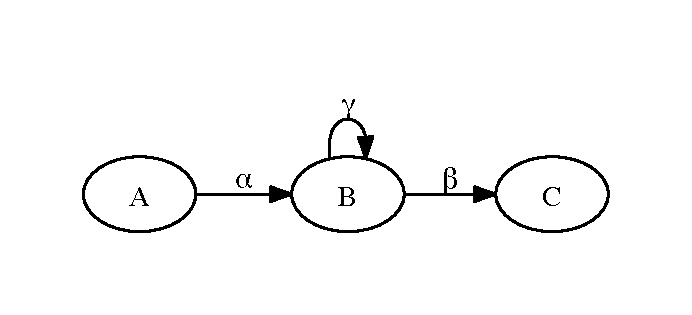
\includegraphics[trim=40 40 40 40,scale=0.6]{images/dfa_re_general}\\
$\alpha\gamma^*\beta$
\end{center}
Which means, if we were to delete state $B$ above, the our new edge from $A$ to
$C$ would be $\alpha\gamma^*\beta$. Note, if $\gamma$ is empty (there's no self loop)
then it's just $\alpha\beta$.

\begin{center}
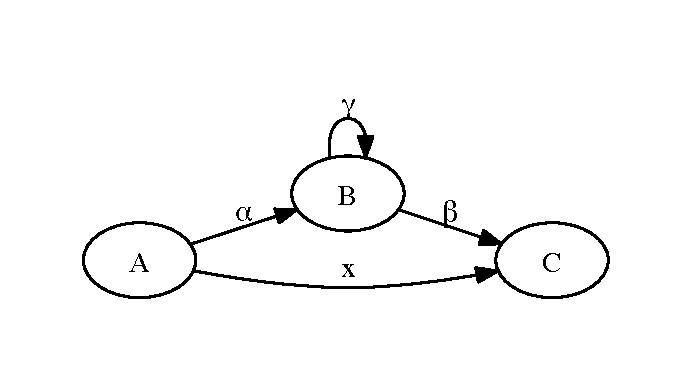
\includegraphics[trim=40 40 40 40,scale=0.6]{images/dfa_re_general2}\\
$x+(\alpha\gamma^*\beta)$
\end{center}
Which means that if we delete state $B$ above, and an edge from $A$ to $C$ exists
already, then the new edge is the union of both the general equation above,
and the existing edge.

% -! DFA minimization
%   - Table-construction algorithm
\subsection{DFA Minimization}

    \subsubsection{Table Conversion Algorithm}
    Draw a table with all states of the DFA on both the $x$ and the $y$ axis.
    Consider all input strings of length $0..n$. Start from a state $s$ on
    the $x$ axis, if an input string of length $n$ reaches a state that is final,
    and a state on the $y$ axis given the same input does not reach a final state
    (or vice versa), then we know that those states are not equal, and their cell
    can be marked off. Once a round of this goes by without any cells being
    marked, then we know that the states corresponding to cells that
    are not marked are equivalent.

    \subsubsection{Brzozowski's Algorithm}
    This algorithm is quite simple. The crux of it is that an NFA to DFA conversion
    naturally results in a minimization of the NFA. So the algorithm is as-follows:
    Take a DFA, reverse it to get an NFA, convert that NFA to a DFA again, take
    this new reversed DFA and reverse it to get the original language back, then
    convert the NFA resulting from the reversal into a DFA.
